\subsection{Architektur}

\subsubsection{Übersicht}
Die strongMan Applikation ist webbasiert, der Aufbau gliedert sich in folgende Komponenten.

\paragraph{Webbrowser} ist der Einstiegspunkt für den Benutzer und übernimmt die Darstellung mithilfe von HTML und CSS. Die Kommunikation findet per HTTP statt. Durch den Einsatz von Javascript wirkt das Arbeiten mit der Oberfläche flüssiger.

\paragraph{Django Server} beinhaltet die eigentliche Business Logik,  stellt dem Webbrowser den Inhalt zur Verfügung, regelt die Kommunikation mit strongSwan per Unix Socket und nutzt zur Persisterung der Daten die Datenbank.

\paragraph{Database} beinhaltet die Konfigurationsangaben, sowie die Zertifikate. Sensitive Daten werden verschlüsselt gespeichert.

\paragraph{strongSwan} baut die IPsec-Tunnels auf und ab. Der Django Server nutzt die VICI-Schnittstelle um Verbindungskonfiguration zu übergeben und die Verbindungen zu starten beziehungsweise zu stoppen. \\\\


\begin{figure}[H]
\centering
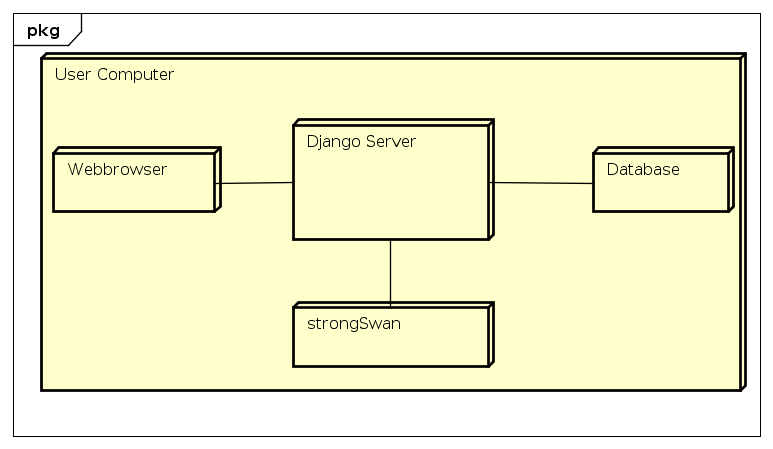
\includegraphics[width=360pt]{images/deployment.png}
\caption[Deployment]{Deployment}
\end{figure}

\subsection{Domain Model}

\begin{figure}[H]
\centering
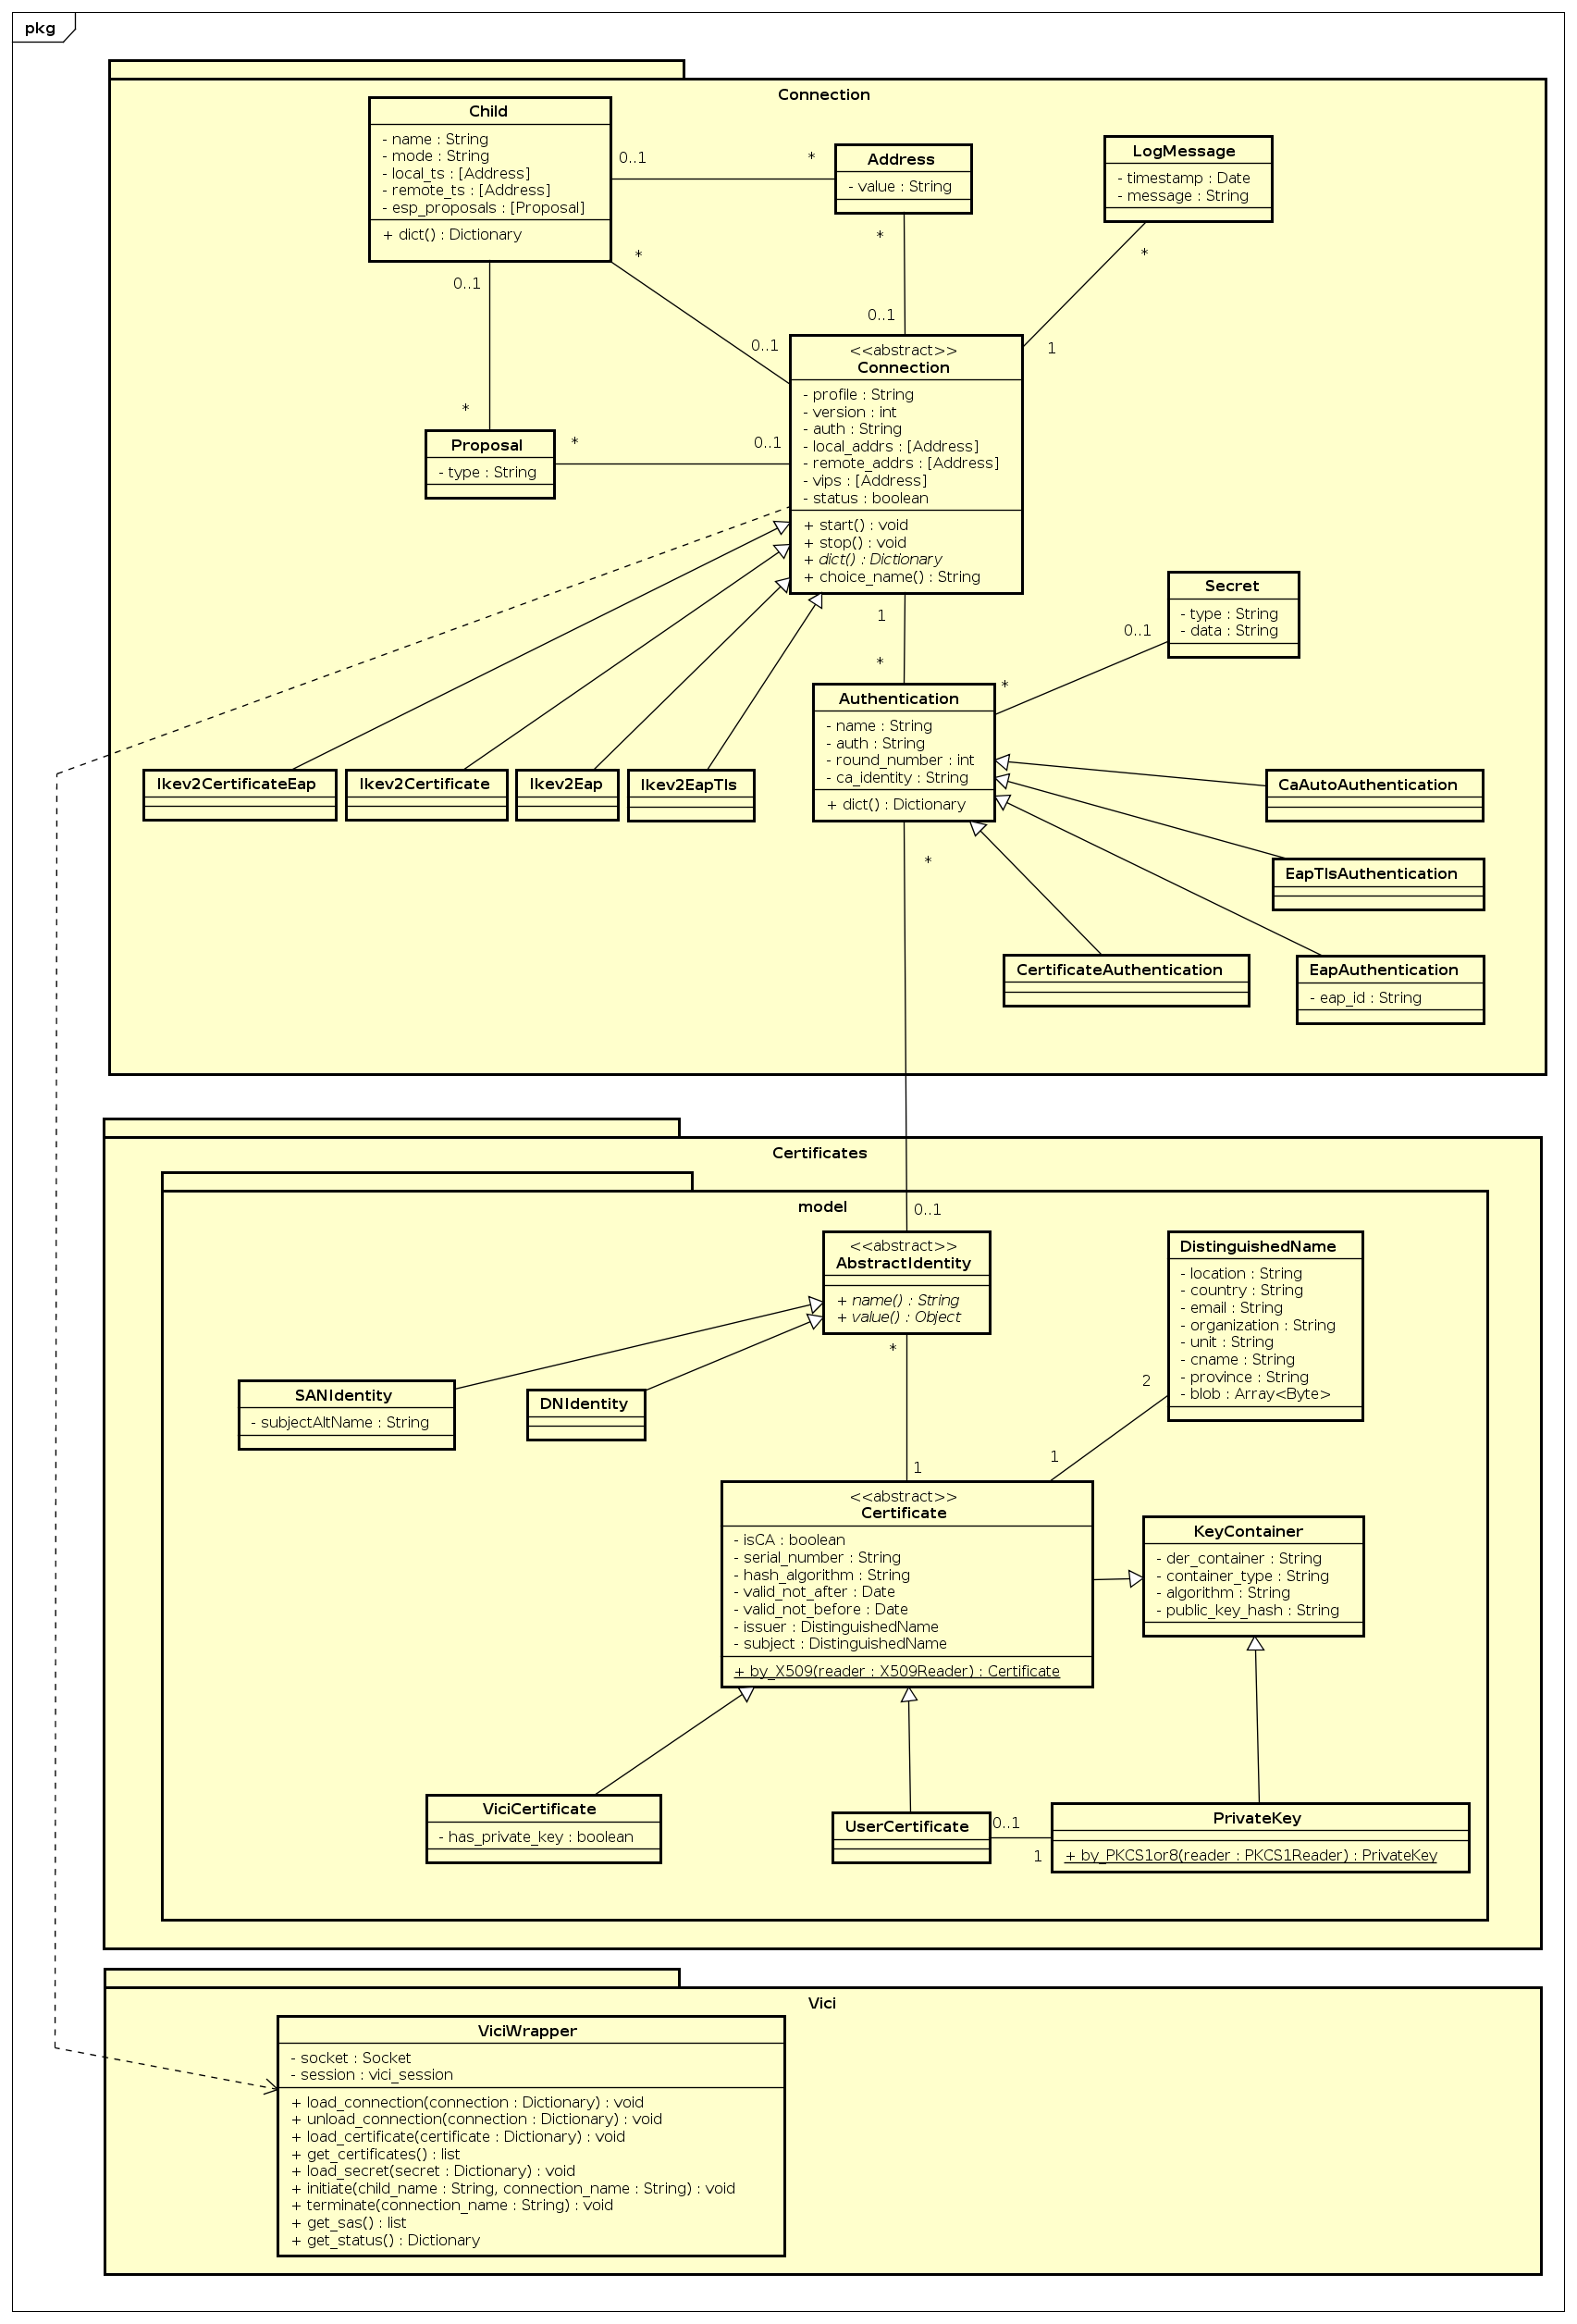
\includegraphics[width=440pt]{images/domain_model.png}
\caption[Domain Model]{Domain Model}
\end{figure}

Das Domain Model teilt sich in drei Teile VICI, Certificates und Connections auf. Diese bauen dabei hierarchisch aufeinander auf.

\subsubsection{VICI}
Das VICI Package beinhaltet den ViciWrapper, der verschiedene Befehle aus der VICI Bibliothek in einen Befehl bündelt, sowie die Exceptions managet. Der Wrapper ist selbst für den Verbindungsauf- und Abbau zuständig.

\subsubsection{Certificates}
Das Package Certificates beinhaltet die Klassen zur Zertifikatsverwaltung. Alle Schlüsselcontainer, die im Uploadfeld hinaufgeladen werden, werden mithilfe des ORM's in dieses Package abgespeichert. Die Hauptklasse des Packages sind UserCertificate, ViciCertificate und PrivateKey.


\par
\begingroup
\leftskip=1.0cm 
\noindent
\paragraph{UserCertificate} Stellt ein X.509 Zertifikat dar, das vom Benutzer hochgeladen wird.
\paragraph{ViciCertificate} Ein X.509 Zertifikat, das aus der VICI-Schnittstelle gelesen wird.
\paragraph{PrivateKey} Privater Schlüssel, der vom Benutzer geuploaded wird und eine Verbindung zum entsprechenden UserCertificate hat.

\paragraph{Identity} Eine Identity ist entweder ein Subject Alternative Name oder ein Distinguished Name. Es dient als Verbindungsstück zum Connection Package

\par
\endgroup



\subsubsection{Connections}
Das Connection Package ist im Allgemeinen eine Abstraktion der VICI-Schnittstelle. Um die verschieden Verbindungstypen abzubilden, wird auf Vererbung gesetzt. Die Methode dict() stellt alle verbindungsrelevanten Einträge aus der Datenbank in einem ordered Dictionary zusammen, welche über den ViciWrapper an strongSwan übergeben werden. Durch start() und stop() werden die übertragenen IPsec Verbindungen auf- und abgebaut.

\par
\begingroup
\leftskip=1.0cm 
\noindent
\paragraph{LogMessage} Wird verwendet um LogMessages über mehrere Requests zu verteilen.

\paragraph{Secret} Bildet die Secret Section der VICI-Schnittstelle ab, dabei wird das Data Feld verschlüsselt in der Datenbank abgelegt. 

\par
\endgroup

\newpage